% Options for packages loaded elsewhere
\PassOptionsToPackage{unicode}{hyperref}
\PassOptionsToPackage{hyphens}{url}
%
\documentclass[
  12pt,
]{article}
\usepackage{lmodern}
\usepackage{amssymb,amsmath}
\usepackage{ifxetex,ifluatex}
\ifnum 0\ifxetex 1\fi\ifluatex 1\fi=0 % if pdftex
  \usepackage[T1]{fontenc}
  \usepackage[utf8]{inputenc}
  \usepackage{textcomp} % provide euro and other symbols
\else % if luatex or xetex
  \usepackage{unicode-math}
  \defaultfontfeatures{Scale=MatchLowercase}
  \defaultfontfeatures[\rmfamily]{Ligatures=TeX,Scale=1}
  \setmainfont[]{Times New Roman}
\fi
% Use upquote if available, for straight quotes in verbatim environments
\IfFileExists{upquote.sty}{\usepackage{upquote}}{}
\IfFileExists{microtype.sty}{% use microtype if available
  \usepackage[]{microtype}
  \UseMicrotypeSet[protrusion]{basicmath} % disable protrusion for tt fonts
}{}
\makeatletter
\@ifundefined{KOMAClassName}{% if non-KOMA class
  \IfFileExists{parskip.sty}{%
    \usepackage{parskip}
  }{% else
    \setlength{\parindent}{0pt}
    \setlength{\parskip}{6pt plus 2pt minus 1pt}}
}{% if KOMA class
  \KOMAoptions{parskip=half}}
\makeatother
\usepackage{xcolor}
\IfFileExists{xurl.sty}{\usepackage{xurl}}{} % add URL line breaks if available
\IfFileExists{bookmark.sty}{\usepackage{bookmark}}{\usepackage{hyperref}}
\hypersetup{
  pdftitle={Birth Outcomes Associated with CAFOs in Different Race},
  pdfauthor={Jared Wang},
  hidelinks,
  pdfcreator={LaTeX via pandoc}}
\urlstyle{same} % disable monospaced font for URLs
\usepackage[margin=2.54cm]{geometry}
\usepackage{color}
\usepackage{fancyvrb}
\newcommand{\VerbBar}{|}
\newcommand{\VERB}{\Verb[commandchars=\\\{\}]}
\DefineVerbatimEnvironment{Highlighting}{Verbatim}{commandchars=\\\{\}}
% Add ',fontsize=\small' for more characters per line
\usepackage{framed}
\definecolor{shadecolor}{RGB}{248,248,248}
\newenvironment{Shaded}{\begin{snugshade}}{\end{snugshade}}
\newcommand{\AlertTok}[1]{\textcolor[rgb]{0.94,0.16,0.16}{#1}}
\newcommand{\AnnotationTok}[1]{\textcolor[rgb]{0.56,0.35,0.01}{\textbf{\textit{#1}}}}
\newcommand{\AttributeTok}[1]{\textcolor[rgb]{0.77,0.63,0.00}{#1}}
\newcommand{\BaseNTok}[1]{\textcolor[rgb]{0.00,0.00,0.81}{#1}}
\newcommand{\BuiltInTok}[1]{#1}
\newcommand{\CharTok}[1]{\textcolor[rgb]{0.31,0.60,0.02}{#1}}
\newcommand{\CommentTok}[1]{\textcolor[rgb]{0.56,0.35,0.01}{\textit{#1}}}
\newcommand{\CommentVarTok}[1]{\textcolor[rgb]{0.56,0.35,0.01}{\textbf{\textit{#1}}}}
\newcommand{\ConstantTok}[1]{\textcolor[rgb]{0.00,0.00,0.00}{#1}}
\newcommand{\ControlFlowTok}[1]{\textcolor[rgb]{0.13,0.29,0.53}{\textbf{#1}}}
\newcommand{\DataTypeTok}[1]{\textcolor[rgb]{0.13,0.29,0.53}{#1}}
\newcommand{\DecValTok}[1]{\textcolor[rgb]{0.00,0.00,0.81}{#1}}
\newcommand{\DocumentationTok}[1]{\textcolor[rgb]{0.56,0.35,0.01}{\textbf{\textit{#1}}}}
\newcommand{\ErrorTok}[1]{\textcolor[rgb]{0.64,0.00,0.00}{\textbf{#1}}}
\newcommand{\ExtensionTok}[1]{#1}
\newcommand{\FloatTok}[1]{\textcolor[rgb]{0.00,0.00,0.81}{#1}}
\newcommand{\FunctionTok}[1]{\textcolor[rgb]{0.00,0.00,0.00}{#1}}
\newcommand{\ImportTok}[1]{#1}
\newcommand{\InformationTok}[1]{\textcolor[rgb]{0.56,0.35,0.01}{\textbf{\textit{#1}}}}
\newcommand{\KeywordTok}[1]{\textcolor[rgb]{0.13,0.29,0.53}{\textbf{#1}}}
\newcommand{\NormalTok}[1]{#1}
\newcommand{\OperatorTok}[1]{\textcolor[rgb]{0.81,0.36,0.00}{\textbf{#1}}}
\newcommand{\OtherTok}[1]{\textcolor[rgb]{0.56,0.35,0.01}{#1}}
\newcommand{\PreprocessorTok}[1]{\textcolor[rgb]{0.56,0.35,0.01}{\textit{#1}}}
\newcommand{\RegionMarkerTok}[1]{#1}
\newcommand{\SpecialCharTok}[1]{\textcolor[rgb]{0.00,0.00,0.00}{#1}}
\newcommand{\SpecialStringTok}[1]{\textcolor[rgb]{0.31,0.60,0.02}{#1}}
\newcommand{\StringTok}[1]{\textcolor[rgb]{0.31,0.60,0.02}{#1}}
\newcommand{\VariableTok}[1]{\textcolor[rgb]{0.00,0.00,0.00}{#1}}
\newcommand{\VerbatimStringTok}[1]{\textcolor[rgb]{0.31,0.60,0.02}{#1}}
\newcommand{\WarningTok}[1]{\textcolor[rgb]{0.56,0.35,0.01}{\textbf{\textit{#1}}}}
\usepackage{graphicx,grffile}
\makeatletter
\def\maxwidth{\ifdim\Gin@nat@width>\linewidth\linewidth\else\Gin@nat@width\fi}
\def\maxheight{\ifdim\Gin@nat@height>\textheight\textheight\else\Gin@nat@height\fi}
\makeatother
% Scale images if necessary, so that they will not overflow the page
% margins by default, and it is still possible to overwrite the defaults
% using explicit options in \includegraphics[width, height, ...]{}
\setkeys{Gin}{width=\maxwidth,height=\maxheight,keepaspectratio}
% Set default figure placement to htbp
\makeatletter
\def\fps@figure{htbp}
\makeatother
\setlength{\emergencystretch}{3em} % prevent overfull lines
\providecommand{\tightlist}{%
  \setlength{\itemsep}{0pt}\setlength{\parskip}{0pt}}
\setcounter{secnumdepth}{5}

\title{Birth Outcomes Associated with CAFOs in Different Race}
\usepackage{etoolbox}
\makeatletter
\providecommand{\subtitle}[1]{% add subtitle to \maketitle
  \apptocmd{\@title}{\par {\large #1 \par}}{}{}
}
\makeatother
\subtitle{\url{https://github.com/cwangjared/ENV872-FINAL-PROJECT.git}}
\author{Jared Wang}
\date{4/24/2020}

\begin{document}
\maketitle

\begin{Shaded}
\begin{Highlighting}[]
\CommentTok{#-----------------------------working directory-----------------------------}
\KeywordTok{getwd}\NormalTok{()}

\CommentTok{#-----------------------------load packages-----------------------------}
\KeywordTok{library}\NormalTok{(tidyverse)}
\KeywordTok{library}\NormalTok{(ggthemes)}
\KeywordTok{library}\NormalTok{(ggplot2)}
\KeywordTok{library}\NormalTok{(tidyr)}
\KeywordTok{library}\NormalTok{(gridExtra)}
\KeywordTok{library}\NormalTok{(nlme)}

\CommentTok{#-----------------------------set ggplot theme-----------------------------}
\NormalTok{theme.hc01 <-}\StringTok{ }\KeywordTok{theme_hc}\NormalTok{() }\OperatorTok{+}
\StringTok{  }\KeywordTok{theme}\NormalTok{(}\DataTypeTok{axis.title =} \KeywordTok{element_text}\NormalTok{(}\DataTypeTok{family =} \StringTok{"serif"}\NormalTok{, }\DataTypeTok{size =}\NormalTok{ (}\DecValTok{10}\NormalTok{)),}
        \DataTypeTok{axis.text =} \KeywordTok{element_text}\NormalTok{(}\DataTypeTok{family =} \StringTok{"serif"}\NormalTok{, }\DataTypeTok{size =}\NormalTok{ (}\DecValTok{8}\NormalTok{), }\DataTypeTok{color =} \StringTok{"black"}\NormalTok{))}

\CommentTok{#-----------------------------load dataset-----------------------------}
\NormalTok{df.birth.temp <-}\StringTok{ }\KeywordTok{read.csv}\NormalTok{(}\StringTok{"../data/raw/birth.csv"}\NormalTok{)}
\end{Highlighting}
\end{Shaded}

\hypertarget{rationale-and-research-questions}{%
\section{Rationale and Research
Questions}\label{rationale-and-research-questions}}

Concentrated animal feeding operations is a significant source of water
and air contaminants in southeastern North Carolina. Contamination from
these facilities poses significant health threats to local communities.
Residents living in areas with more CAFOs tend to have higher odds for
adverse health outcomes such as respiratory disease and kidney disease.
My Masters' Project investigated assocatiation between proximity to
CAFOs and infant birth outcomes (gestational age and birth weight). In
the past project, I identified that higher hog density and larger hog
size are associated with smaller gestational age and birth weight.

While the Masters' Project focuses on impact of CAFOs on the general
population, it only take race as a confounding variable. However,
certain races, such as Black and Latino, are usually more strongly
impacted by adverse environmental conditions than other races. For this
project, I am interested in exploring if a certain race is
disproportionally vulnerable to CAFOs. This project aims to use
generalized linear model to explore association between hog CAFO kernel
density score (explained in the next section) and birth outcomes
(gestational age \& birth weight), stratified by race.

The research question is: is the relationship between hog CAFO kernel
density scores and birth outcomes the same among different races?

\newpage

\hypertarget{dataset-information}{%
\section{Dataset Information}\label{dataset-information}}

Predictor: hog CAFO kernel density score (represents impact from hog
CAFOs) Birth outcomes: birth weight \& gestational age Confouding
variables: infant sex, maternal age, education, smoking history, BMI,
and marital status

This project uses 1) NC household level demographic and birth outcome
dataset in 2016 and 2) hog CAFO kernel density scores. Both datasets are
used in and wrangled for the purpose of my Masters' Project. In this
project, I take the dataset wrangled for my MP and modify it to make it
fit this project.

The demographic and birth outcome dataset is obtained from the NC birth
certificate dataset (confidential information excluded). The dataset
include the following variables: birth weight, gestational age, infant
sex, mother's age, prenatal BMI, smoking history, prenatal care index
level, naternal race, and maternal education.

Kernel density score reflects relative impact of hog CAFOs on each
houeshold (each household has a unique score). It is calculated from
numbers of hog CAFOs in 5 mi radius region, animal count in each CAFO,
and animal size in each CAFO. The computation is completed by the Kernel
Density tool in ArcGIS. The GIS model was completed as a part of the MP.
Results are previously merged with the birth certificate dataset (code
included below).

\begin{Shaded}
\begin{Highlighting}[]
\CommentTok{#----------------------------data wrangling completed as a part of MP-----------------------------}
\NormalTok{df.birth <-}\StringTok{ }\NormalTok{df.birth.temp }\OperatorTok
\StringTok{  }\KeywordTok{select}\NormalTok{(KID, GEST, LBS, OZS, SEX, MARITAL, CIGPN, }\CommentTok{#select explanatory variables}
\NormalTok{         CIGFN, CIGSN, CIGLN, MEDUC, MRACE, MHISP, }
\NormalTok{         KOTEL, MAGE, BMI, PLUR, Poul1, Poul2, Poul5, }
\NormalTok{         Hog1, Hog2, Hog5, gridcodehog, gridcodepol) }\OperatorTok
\StringTok{  }\KeywordTok{mutate}\NormalTok{(}\DataTypeTok{HOG1 =}\NormalTok{ Hog1, }\DataTypeTok{HOG2 =}\NormalTok{ Hog2, }\DataTypeTok{HOG5 =}\NormalTok{ Hog5, }
         \DataTypeTok{POU1 =}\NormalTok{ Poul1, }\DataTypeTok{POU2 =}\NormalTok{ Poul2, }\DataTypeTok{POU5 =}\NormalTok{ Poul5, }
         \DataTypeTok{EFFHOG =}\NormalTok{ gridcodehog, }\DataTypeTok{EFFPOU =}\NormalTok{ gridcodepol) }\OperatorTok
\StringTok{  }\KeywordTok{select}\NormalTok{(}\OperatorTok{-}\NormalTok{Hog1, }\OperatorTok{-}\NormalTok{Hog2, }\OperatorTok{-}\NormalTok{Hog5, }\OperatorTok{-}\NormalTok{Poul1, }\OperatorTok{-}\NormalTok{Poul2, }\OperatorTok{-}\NormalTok{Poul5, }
         \OperatorTok{-}\NormalTok{gridcodehog, }\OperatorTok{-}\NormalTok{gridcodepol) }\OperatorTok
\StringTok{  }\KeywordTok{filter}\NormalTok{(PLUR }\OperatorTok{==}\StringTok{ }\DecValTok{1}\NormalTok{) }\OperatorTok
\StringTok{  }\KeywordTok{mutate}\NormalTok{(}\DataTypeTok{SEX =} \KeywordTok{ifelse}\NormalTok{(SEX }\OperatorTok{==}\StringTok{ }\DecValTok{9}\NormalTok{, }\OtherTok{NA}\NormalTok{, SEX),}
         \DataTypeTok{MARITAL =} \KeywordTok{ifelse}\NormalTok{(MARITAL }\OperatorTok{==}\StringTok{ }\DecValTok{9}\NormalTok{, }\OtherTok{NA}\NormalTok{, MARITAL),}
         \DataTypeTok{CIGPN =} \KeywordTok{ifelse}\NormalTok{(CIGPN }\OperatorTok{==}\StringTok{ }\DecValTok{99}\NormalTok{, }\OtherTok{NA}\NormalTok{, CIGPN),}
         \DataTypeTok{CIGLN =} \KeywordTok{ifelse}\NormalTok{(CIGLN }\OperatorTok{==}\StringTok{ }\DecValTok{99}\NormalTok{, }\OtherTok{NA}\NormalTok{, CIGLN),}
         \DataTypeTok{CIGSN =} \KeywordTok{ifelse}\NormalTok{(CIGSN }\OperatorTok{==}\StringTok{ }\DecValTok{99}\NormalTok{, }\OtherTok{NA}\NormalTok{, CIGSN),}
         \DataTypeTok{CIGFN =} \KeywordTok{ifelse}\NormalTok{(CIGFN }\OperatorTok{==}\StringTok{ }\DecValTok{99}\NormalTok{, }\OtherTok{NA}\NormalTok{, CIGFN),}
         \DataTypeTok{MEDUC =} \KeywordTok{ifelse}\NormalTok{(MEDUC }\OperatorTok{==}\StringTok{ }\DecValTok{9}\NormalTok{, }\OtherTok{NA}\NormalTok{, MEDUC),}
         \DataTypeTok{KOTEL =} \KeywordTok{ifelse}\NormalTok{(KOTEL }\OperatorTok{==}\StringTok{ }\DecValTok{0}\NormalTok{, }\OtherTok{NA}\NormalTok{, KOTEL),}
         \DataTypeTok{BMI =} \KeywordTok{ifelse}\NormalTok{(BMI }\OperatorTok{==}\StringTok{ }\DecValTok{999}\NormalTok{, }\OtherTok{NA}\NormalTok{, BMI)) }\OperatorTok
\StringTok{  }\KeywordTok{mutate}\NormalTok{(}\DataTypeTok{ERROR =} \KeywordTok{ifelse}\NormalTok{(MAGE }\OperatorTok{==}\StringTok{ }\DecValTok{29} \OperatorTok{&}\StringTok{ }\NormalTok{BMI }\OperatorTok{==}\StringTok{ }\FloatTok{25.7}\NormalTok{, }\DecValTok{1}\NormalTok{, }\DecValTok{0}\NormalTok{),}
         \DataTypeTok{ERROR =} \KeywordTok{as.factor}\NormalTok{(ERROR),}
         \DataTypeTok{ERROR.GEST40 =} \KeywordTok{ifelse}\NormalTok{(ERROR }\OperatorTok{==}\StringTok{ }\DecValTok{1} \OperatorTok{&}\StringTok{ }\NormalTok{GEST }\OperatorTok{==}\StringTok{ }\DecValTok{40}\NormalTok{, }\DecValTok{1}\NormalTok{, }\DecValTok{0}\NormalTok{),}
         \DataTypeTok{ERROR.GEST40 =} \KeywordTok{as.factor}\NormalTok{(ERROR.GEST40)) }\OperatorTok
\StringTok{  }\KeywordTok{select}\NormalTok{(}\OperatorTok{-}\NormalTok{PLUR) }\OperatorTok
\StringTok{  }\KeywordTok{mutate}\NormalTok{(}\DataTypeTok{HOG1 =} \KeywordTok{as.factor}\NormalTok{(HOG1), }\CommentTok{#create 1 mi, 2 mi, and 5 mi distance zones }
         \DataTypeTok{HOG2 =} \KeywordTok{as.factor}\NormalTok{(HOG2),}
         \DataTypeTok{HOG5 =} \KeywordTok{as.factor}\NormalTok{(HOG5),}
         \DataTypeTok{POU1 =} \KeywordTok{as.factor}\NormalTok{(POU1), }
         \DataTypeTok{POU2 =} \KeywordTok{as.factor}\NormalTok{(POU2),}
         \DataTypeTok{POU5 =} \KeywordTok{as.factor}\NormalTok{(POU5),}
         \DataTypeTok{DSTHOG =} \KeywordTok{ifelse}\NormalTok{(HOG5 }\OperatorTok{==}\StringTok{ "1"} \OperatorTok{&}\StringTok{ }\NormalTok{HOG2 }\OperatorTok{==}\StringTok{ "0"} \OperatorTok{&}\StringTok{ }\NormalTok{HOG1 }\OperatorTok{==}\StringTok{ "0"}\NormalTok{, }\StringTok{"x5"}\NormalTok{, }\OtherTok{NA}\NormalTok{),}
         \DataTypeTok{DSTHOG =} \KeywordTok{ifelse}\NormalTok{(HOG2 }\OperatorTok{==}\StringTok{ "1"} \OperatorTok{&}\StringTok{ }\NormalTok{HOG1 }\OperatorTok{==}\StringTok{ "0"}\NormalTok{, }\StringTok{"x2"}\NormalTok{, DSTHOG),}
         \DataTypeTok{DSTHOG =} \KeywordTok{ifelse}\NormalTok{(HOG1 }\OperatorTok{==}\StringTok{ "1"}\NormalTok{, }\StringTok{"x1"}\NormalTok{, DSTHOG),}
         \DataTypeTok{DSTHOG =} \KeywordTok{ifelse}\NormalTok{(HOG5 }\OperatorTok{==}\StringTok{ "0"}\NormalTok{, }\StringTok{"x0"}\NormalTok{, DSTHOG),}
         \DataTypeTok{DSTHOG =} \KeywordTok{as.factor}\NormalTok{(DSTHOG),}
         \DataTypeTok{DSTPOU =} \KeywordTok{ifelse}\NormalTok{(POU5 }\OperatorTok{==}\StringTok{ "1"} \OperatorTok{&}\StringTok{ }\NormalTok{POU2 }\OperatorTok{==}\StringTok{ "0"} \OperatorTok{&}\StringTok{ }\NormalTok{POU1 }\OperatorTok{==}\StringTok{ "0"}\NormalTok{, }\StringTok{"x5"}\NormalTok{, }\OtherTok{NA}\NormalTok{),}
         \DataTypeTok{DSTPOU =} \KeywordTok{ifelse}\NormalTok{(POU2 }\OperatorTok{==}\StringTok{ "1"} \OperatorTok{&}\StringTok{ }\NormalTok{POU1 }\OperatorTok{==}\StringTok{ "0"}\NormalTok{, }\StringTok{"x2"}\NormalTok{, DSTPOU),}
         \DataTypeTok{DSTPOU =} \KeywordTok{ifelse}\NormalTok{(POU1 }\OperatorTok{==}\StringTok{ "1"}\NormalTok{, }\StringTok{"x1"}\NormalTok{, DSTPOU),}
         \DataTypeTok{DSTPOU =} \KeywordTok{ifelse}\NormalTok{(POU5 }\OperatorTok{==}\StringTok{ "0"}\NormalTok{, }\StringTok{"x0"}\NormalTok{, DSTPOU),}
         \DataTypeTok{DSTPOU =} \KeywordTok{as.factor}\NormalTok{(DSTPOU)) }\OperatorTok
\StringTok{  }\KeywordTok{mutate}\NormalTok{(}\DataTypeTok{LBS =} \KeywordTok{ifelse}\NormalTok{(LBS }\OperatorTok{==}\StringTok{ }\DecValTok{99}\NormalTok{, }\OtherTok{NA}\NormalTok{, LBS), }\CommentTok{#convert birth weight to kilogram}
         \DataTypeTok{OZS =} \KeywordTok{ifelse}\NormalTok{(OZS }\OperatorTok{==}\StringTok{ }\DecValTok{99}\NormalTok{, }\OtherTok{NA}\NormalTok{, OZS),}
         \DataTypeTok{lbs_kg =}\NormalTok{ LBS}\OperatorTok{/}\FloatTok{2.205}\NormalTok{,}
         \DataTypeTok{ozs_kg =}\NormalTok{ OZS}\OperatorTok{/}\FloatTok{35.274}\NormalTok{,}
         \DataTypeTok{WTKG =}\NormalTok{ lbs_kg }\OperatorTok{+}\StringTok{ }\NormalTok{ozs_kg) }\OperatorTok
\StringTok{  }\KeywordTok{select}\NormalTok{(}\OperatorTok{-}\NormalTok{lbs_kg, }\OperatorTok{-}\NormalTok{ozs_kg, }\OperatorTok{-}\NormalTok{LBS, }\OperatorTok{-}\NormalTok{OZS) }\OperatorTok\StringTok{ }\CommentTok{#delete used columns}
\StringTok{  }\KeywordTok{mutate}\NormalTok{(}\DataTypeTok{NUMSMOKE =}\NormalTok{ CIGPN }\OperatorTok{+}\StringTok{ }\NormalTok{CIGLN }\OperatorTok{+}\StringTok{ }\NormalTok{CIGSN }\OperatorTok{+}\StringTok{ }\NormalTok{CIGFN,}
         \DataTypeTok{SMOKE =} \KeywordTok{ifelse}\NormalTok{(NUMSMOKE }\OperatorTok{!=}\StringTok{ }\DecValTok{0}\NormalTok{, }\DecValTok{1}\NormalTok{, }\DecValTok{2}\NormalTok{),}
         \DataTypeTok{SMOKE =} \KeywordTok{as.factor}\NormalTok{(SMOKE)) }\OperatorTok
\StringTok{  }\KeywordTok{select}\NormalTok{(}\OperatorTok{-}\NormalTok{CIGPN, }\OperatorTok{-}\NormalTok{CIGLN, }\OperatorTok{-}\NormalTok{CIGSN, }\OperatorTok{-}\StringTok{ }\NormalTok{CIGFN, }\OperatorTok{-}\NormalTok{NUMSMOKE) }\OperatorTok
\StringTok{  }\KeywordTok{mutate}\NormalTok{(}\DataTypeTok{MEDUC =} \KeywordTok{ifelse}\NormalTok{(MEDUC }\OperatorTok\StringTok{ }\KeywordTok{c}\NormalTok{(}\DecValTok{1}\NormalTok{, }\DecValTok{2}\NormalTok{, }\DecValTok{3}\NormalTok{), }\DecValTok{1}\NormalTok{, MEDUC),}
         \DataTypeTok{MEDUC =} \KeywordTok{ifelse}\NormalTok{(MEDUC }\OperatorTok\StringTok{ }\KeywordTok{c}\NormalTok{(}\DecValTok{4}\NormalTok{, }\DecValTok{5}\NormalTok{), }\DecValTok{2}\NormalTok{, MEDUC),}
         \DataTypeTok{MEDUC =} \KeywordTok{ifelse}\NormalTok{(MEDUC }\OperatorTok{==}\StringTok{ }\DecValTok{6}\NormalTok{, }\DecValTok{3}\NormalTok{, MEDUC),}
         \DataTypeTok{MEDUC =} \KeywordTok{ifelse}\NormalTok{(MEDUC }\OperatorTok\StringTok{ }\KeywordTok{c}\NormalTok{(}\DecValTok{7}\NormalTok{, }\DecValTok{8}\NormalTok{), }\DecValTok{4}\NormalTok{, MEDUC)) }\OperatorTok
\StringTok{  }\KeywordTok{mutate}\NormalTok{(}\DataTypeTok{SEX =} \KeywordTok{as.factor}\NormalTok{(SEX), }\CommentTok{#convert variables to factors}
         \DataTypeTok{MARITAL =} \KeywordTok{as.factor}\NormalTok{(MARITAL),}
         \DataTypeTok{MEDUC =} \KeywordTok{as.factor}\NormalTok{(MEDUC),}
         \DataTypeTok{KOTEL =} \KeywordTok{as.factor}\NormalTok{(KOTEL),}
         \DataTypeTok{MRACE =} \KeywordTok{as.factor}\NormalTok{(MRACE),}
         \DataTypeTok{MHISP =} \KeywordTok{as.factor}\NormalTok{(MHISP)) }\OperatorTok
\StringTok{  }\KeywordTok{mutate}\NormalTok{(}\DataTypeTok{MRACE =} \KeywordTok{ifelse}\NormalTok{(MHISP }\OperatorTok\StringTok{ }\KeywordTok{c}\NormalTok{(}\StringTok{"C"}\NormalTok{, }\StringTok{"M"}\NormalTok{, }\StringTok{"O"}\NormalTok{, }\StringTok{"P"}\NormalTok{, }\StringTok{"S"}\NormalTok{), }\StringTok{"H"}\NormalTok{, MRACE), }\CommentTok{#collapse race}
         \DataTypeTok{MRACE =} \KeywordTok{ifelse}\NormalTok{(MRACE }\OperatorTok{==}\StringTok{ "2"}\NormalTok{, }\StringTok{"W"}\NormalTok{, MRACE),}
         \DataTypeTok{MRACE =} \KeywordTok{ifelse}\NormalTok{(MRACE }\OperatorTok{==}\StringTok{ "3"}\NormalTok{, }\StringTok{"B"}\NormalTok{, MRACE),}
         \DataTypeTok{MRACE =} \KeywordTok{ifelse}\NormalTok{(MRACE }\OperatorTok\StringTok{ }\KeywordTok{c}\NormalTok{(}\StringTok{"1"}\NormalTok{, }\StringTok{"4"}\NormalTok{, }\StringTok{"5"}\NormalTok{, }\StringTok{"6"}\NormalTok{, }\StringTok{"7"}\NormalTok{, }\StringTok{"8"}\NormalTok{, }\StringTok{"9"}\NormalTok{), }\StringTok{"O"}\NormalTok{, MRACE),}
         \DataTypeTok{MRACE =} \KeywordTok{as.factor}\NormalTok{(MRACE)) }\OperatorTok
\StringTok{  }\KeywordTok{select}\NormalTok{(}\OperatorTok{-}\NormalTok{MHISP) }\OperatorTok
\StringTok{  }\KeywordTok{mutate}\NormalTok{(}\DataTypeTok{GEST =} \KeywordTok{ifelse}\NormalTok{(GEST }\OperatorTok{==}\StringTok{ }\DecValTok{99}\NormalTok{, }\OtherTok{NA}\NormalTok{, GEST), }\CommentTok{#clean gestational age values}
         \DataTypeTok{PRETERM =} \KeywordTok{ifelse}\NormalTok{(GEST }\OperatorTok{<}\StringTok{ }\DecValTok{37}\NormalTok{, }\StringTok{"1"}\NormalTok{, }\StringTok{"0"}\NormalTok{),}
         \DataTypeTok{PRETERM =} \KeywordTok{as.factor}\NormalTok{(PRETERM),}
         \DataTypeTok{WTKG =} \KeywordTok{ifelse}\NormalTok{(WTKG }\OperatorTok{>}\StringTok{ }\DecValTok{7}\NormalTok{, }\OtherTok{NA}\NormalTok{, WTKG),}
         \DataTypeTok{WTKG =} \KeywordTok{ifelse}\NormalTok{(WTKG }\OperatorTok{<}\StringTok{ }\FloatTok{0.1}\NormalTok{, }\OtherTok{NA}\NormalTok{, WTKG),}
         \DataTypeTok{LBW =} \KeywordTok{ifelse}\NormalTok{(WTKG }\OperatorTok{<}\StringTok{ }\FloatTok{2.5}\NormalTok{, }\StringTok{"1"}\NormalTok{, }\StringTok{"0"}\NormalTok{),}
         \DataTypeTok{LBW =} \KeywordTok{as.factor}\NormalTok{(LBW)) }\OperatorTok\StringTok{ }\CommentTok{#clean birth weight values}
\StringTok{  }\KeywordTok{na.omit}\NormalTok{()}
\end{Highlighting}
\end{Shaded}

The dataset used for MP is almost ready for this analysis. To simplify
the dataset, the following wrangling approach is used. The ten variables
used in this analysis is selected and renamed. Then variables are
recoded. The dataset covers the entire state of NC, while kernel density
analysis is only applicable for households living within 5 mi from a hog
CAFO. Therefore, all zero values for kernel density should be
eliminated.

\begin{Shaded}
\begin{Highlighting}[]
\NormalTok{df.birth.kernel <-}\StringTok{ }\NormalTok{df.birth }\OperatorTok
\StringTok{  }\KeywordTok{select}\NormalTok{(GEST, WTKG, EFFHOG, MARITAL, SEX, MAGE, }
\NormalTok{         MEDUC, MRACE, KOTEL, BMI) }\OperatorTok\StringTok{ }\CommentTok{#select desired variables}
\StringTok{  }\KeywordTok{mutate}\NormalTok{(}\DataTypeTok{gestational.age =}\NormalTok{ GEST, }\DataTypeTok{birth.weight =}\NormalTok{ WTKG, }
         \DataTypeTok{kernel.score =}\NormalTok{ EFFHOG, }\DataTypeTok{marital.status =}\NormalTok{ MARITAL, }
         \DataTypeTok{infant.sex =}\NormalTok{ SEX, }\DataTypeTok{mother.age =}\NormalTok{ MAGE, }
         \DataTypeTok{education =}\NormalTok{ MEDUC, }\DataTypeTok{race =}\NormalTok{ MRACE, }
         \DataTypeTok{prenatal.care =}\NormalTok{ KOTEL) }\OperatorTok
\StringTok{  }\KeywordTok{mutate}\NormalTok{(}\DataTypeTok{marital.status =} \KeywordTok{ifelse}\NormalTok{(marital.status }\OperatorTok{==}\StringTok{ }\DecValTok{1}\NormalTok{, }\StringTok{"married"}\NormalTok{, }\StringTok{"single"}\NormalTok{), }\CommentTok{#recode variables}
         \DataTypeTok{marital.status =} \KeywordTok{as.factor}\NormalTok{(marital.status), }
         \DataTypeTok{infant.sex =} \KeywordTok{ifelse}\NormalTok{(infant.sex }\OperatorTok{==}\StringTok{ }\DecValTok{1}\NormalTok{, }\StringTok{"male"}\NormalTok{, }\StringTok{"female"}\NormalTok{), }
         \DataTypeTok{infant.sex =} \KeywordTok{as.factor}\NormalTok{(infant.sex), }
         \DataTypeTok{prenatal.care =} \KeywordTok{as.factor}\NormalTok{(prenatal.care), }
         \DataTypeTok{education =} \KeywordTok{ifelse}\NormalTok{(education }\OperatorTok{==}\StringTok{ }\DecValTok{1}\NormalTok{, }\StringTok{"highschool.below"}\NormalTok{, education), }
         \DataTypeTok{education =} \KeywordTok{ifelse}\NormalTok{(education }\OperatorTok{==}\StringTok{ }\DecValTok{2}\NormalTok{, }\StringTok{"some.college"}\NormalTok{, education), }
         \DataTypeTok{education =} \KeywordTok{ifelse}\NormalTok{(education }\OperatorTok{==}\StringTok{ }\DecValTok{3}\NormalTok{, }\StringTok{"complete.college"}\NormalTok{, education), }
         \DataTypeTok{education =} \KeywordTok{ifelse}\NormalTok{(education }\OperatorTok{==}\StringTok{ }\DecValTok{4}\NormalTok{, }\StringTok{"graduate"}\NormalTok{, education), }
         \DataTypeTok{education =} \KeywordTok{as.factor}\NormalTok{(education), }
         \DataTypeTok{race =} \KeywordTok{as.factor}\NormalTok{(race)) }\OperatorTok
\StringTok{  }\KeywordTok{select}\NormalTok{(}\OperatorTok{-}\NormalTok{GEST, }\OperatorTok{-}\NormalTok{WTKG, }\OperatorTok{-}\NormalTok{EFFHOG, }\OperatorTok{-}\NormalTok{MARITAL, }\OperatorTok{-}\NormalTok{SEX, }\OperatorTok{-}\NormalTok{MAGE, }
         \OperatorTok{-}\NormalTok{MEDUC, }\OperatorTok{-}\NormalTok{MRACE, }\OperatorTok{-}\NormalTok{KOTEL) }\OperatorTok
\StringTok{  }\KeywordTok{filter}\NormalTok{(kernel.score }\OperatorTok{!=}\StringTok{ }\DecValTok{0}\NormalTok{)}

\CommentTok{#-----------------------export the dataset-----------------}
\KeywordTok{write.csv}\NormalTok{(df.birth.kernel, }\StringTok{"../data/processed/birth.kernel.csv"}\NormalTok{)}
\end{Highlighting}
\end{Shaded}

\newpage

\hypertarget{exploratory-analysis}{%
\section{Exploratory Analysis}\label{exploratory-analysis}}

In general, distribution of kernel scores is skewed and data
transformation may be needed. The report is associated with some other
values. The total number is large.

\begin{Shaded}
\begin{Highlighting}[]
\KeywordTok{summary}\NormalTok{(df.birth.kernel)}
\end{Highlighting}
\end{Shaded}

\begin{verbatim}
##       BMI        gestational.age  birth.weight     kernel.score   
##  Min.   : 7.90   Min.   :17.0    Min.   :0.1701   Min.   :   1.0  
##  1st Qu.:22.50   1st Qu.:38.0    1st Qu.:2.9762   1st Qu.:  11.0  
##  Median :26.40   Median :39.0    Median :3.3164   Median :  42.0  
##  Mean   :27.83   Mean   :38.6    Mean   :3.2774   Mean   : 160.4  
##  3rd Qu.:31.80   3rd Qu.:40.0    3rd Qu.:3.6565   3rd Qu.: 169.0  
##  Max.   :66.80   Max.   :43.0    Max.   :6.0374   Max.   :4864.0  
##  marital.status   infant.sex      mother.age               education   
##  married:10693   female: 9820   Min.   :11.00   complete.college:2842  
##  single : 9452   male  :10325   1st Qu.:23.00   graduate        :1217  
##                                 Median :27.00   highschool.below:8734  
##                                 Mean   :27.29   some.college    :7352  
##                                 3rd Qu.:31.00                          
##                                 Max.   :53.00                          
##  race      prenatal.care
##  B: 5633   1:3916       
##  H: 3199   2:1359       
##  O: 1101   3:5618       
##  W:10212   4:9252       
##                         
## 
\end{verbatim}

In general, distribution of birth weight and gestational age values fit
normal distribution, while that of kernel density does not. Natural
logarithm is therefore applied to transform the kernel density data.
Natural-log-transformed kernel density score generally fits normal
distribution (Figure 1).

\begin{Shaded}
\begin{Highlighting}[]
\NormalTok{hist.bw <-}\StringTok{ }\KeywordTok{ggplot}\NormalTok{(df.birth.kernel) }\OperatorTok{+}
\StringTok{  }\KeywordTok{geom_histogram}\NormalTok{(}\KeywordTok{aes}\NormalTok{(birth.weight), }\DataTypeTok{binwidth =} \FloatTok{0.025}\NormalTok{, }\DataTypeTok{fill =} \StringTok{"lightskyblue4"}\NormalTok{) }\OperatorTok{+}
\StringTok{  }\KeywordTok{labs}\NormalTok{(}\DataTypeTok{y=} \StringTok{"# Household"}\NormalTok{, }\DataTypeTok{x =} \StringTok{"Birth weight (kg)"}\NormalTok{) }\OperatorTok{+}\StringTok{ }
\StringTok{  }\NormalTok{theme.hc01}

\NormalTok{hist.gest <-}\StringTok{ }\KeywordTok{ggplot}\NormalTok{(df.birth.kernel) }\OperatorTok{+}
\StringTok{  }\KeywordTok{geom_histogram}\NormalTok{(}\KeywordTok{aes}\NormalTok{(gestational.age), }\DataTypeTok{binwidth =} \DecValTok{1}\NormalTok{, }\DataTypeTok{fill =} \StringTok{"lightskyblue4"}\NormalTok{) }\OperatorTok{+}
\StringTok{  }\KeywordTok{labs}\NormalTok{(}\DataTypeTok{y=} \StringTok{"# Household"}\NormalTok{, }\DataTypeTok{x =} \StringTok{"Gestational age (weeks)"}\NormalTok{) }\OperatorTok{+}\StringTok{ }
\StringTok{  }\NormalTok{theme.hc01}

\NormalTok{hist.kern <-}\StringTok{ }\KeywordTok{ggplot}\NormalTok{(df.birth.kernel) }\OperatorTok{+}
\StringTok{  }\KeywordTok{geom_histogram}\NormalTok{(}\KeywordTok{aes}\NormalTok{(kernel.score), }\DataTypeTok{binwidth =} \DecValTok{1}\NormalTok{, }\DataTypeTok{fill =} \StringTok{"lightskyblue4"}\NormalTok{) }\OperatorTok{+}\StringTok{ }
\StringTok{  }\KeywordTok{scale_y_continuous}\NormalTok{(}\DataTypeTok{limits =} \KeywordTok{c}\NormalTok{(}\DecValTok{0}\NormalTok{, }\DecValTok{300}\NormalTok{)) }\OperatorTok{+}\StringTok{ }
\StringTok{  }\KeywordTok{labs}\NormalTok{(}\DataTypeTok{y=} \StringTok{"# Household"}\NormalTok{, }\DataTypeTok{x =} \StringTok{"Kernel density score"}\NormalTok{) }\OperatorTok{+}\StringTok{ }
\StringTok{  }\NormalTok{theme.hc01}

\NormalTok{df.birth.kernel <-}\StringTok{ }\NormalTok{df.birth.kernel }\OperatorTok
\StringTok{  }\KeywordTok{mutate}\NormalTok{(}\DataTypeTok{kernel.score.log =} \KeywordTok{log}\NormalTok{(kernel.score))}

\NormalTok{hist.kernlog <-}\StringTok{ }\KeywordTok{ggplot}\NormalTok{(df.birth.kernel) }\OperatorTok{+}
\StringTok{  }\KeywordTok{geom_histogram}\NormalTok{(}\KeywordTok{aes}\NormalTok{(kernel.score.log), }\DataTypeTok{binwidth =} \DecValTok{1}\NormalTok{, }\DataTypeTok{fill =} \StringTok{"lightskyblue4"}\NormalTok{) }\OperatorTok{+}
\StringTok{  }\KeywordTok{labs}\NormalTok{(}\DataTypeTok{y=} \StringTok{"# Household"}\NormalTok{, }\DataTypeTok{x =} \StringTok{"Log kernel density score"}\NormalTok{) }\OperatorTok{+}\StringTok{ }
\StringTok{  }\NormalTok{theme.hc01}

\KeywordTok{grid.arrange}\NormalTok{(hist.bw, hist.gest, }
\NormalTok{             hist.kern, hist.kernlog, }\DataTypeTok{ncol =} \DecValTok{2}\NormalTok{)}
\end{Highlighting}
\end{Shaded}

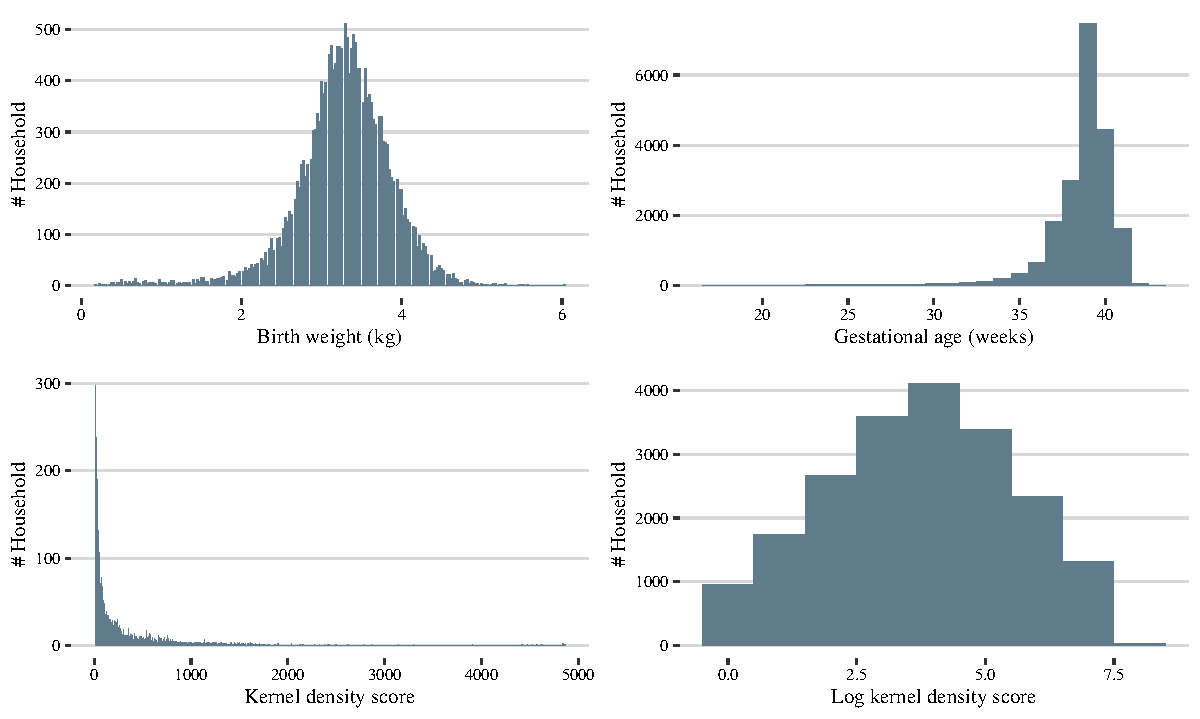
\includegraphics{ENV872_FINAL_CW_files/figure-latex/unnamed-chunk-5-1.pdf}
Figure 1: visualization of birth weight, gestational age, and hog CAFO
kernel density scores.

It is difficult to conclude a general trend from visualized data.
However, there appear to be difference between average birth weight
among different race. For example, white and hispanic infants tend to
have higher average birth weight than black infants (Figure 2).

\begin{Shaded}
\begin{Highlighting}[]
\CommentTok{#create four datasets}
\NormalTok{df.black <-}\StringTok{ }\NormalTok{df.birth.kernel }\OperatorTok
\StringTok{  }\KeywordTok{filter}\NormalTok{(race }\OperatorTok{==}\StringTok{ "B"}\NormalTok{)}
\NormalTok{df.hisp <-}\StringTok{ }\NormalTok{df.birth.kernel }\OperatorTok
\StringTok{  }\KeywordTok{filter}\NormalTok{(race }\OperatorTok{==}\StringTok{ "H"}\NormalTok{)}
\NormalTok{df.white <-}\StringTok{ }\NormalTok{df.birth.kernel }\OperatorTok
\StringTok{  }\KeywordTok{filter}\NormalTok{(race }\OperatorTok{==}\StringTok{ "W"}\NormalTok{)}
\NormalTok{df.other <-}\StringTok{ }\NormalTok{df.birth.kernel }\OperatorTok
\StringTok{  }\KeywordTok{filter}\NormalTok{(race }\OperatorTok{==}\StringTok{ "O"}\NormalTok{)}

\CommentTok{#plot}
\NormalTok{scat.bw.black <-}\StringTok{ }\KeywordTok{ggplot}\NormalTok{(df.black) }\OperatorTok{+}
\StringTok{  }\KeywordTok{geom_point}\NormalTok{(}\KeywordTok{aes}\NormalTok{(}\DataTypeTok{x =}\NormalTok{ kernel.score.log, }\DataTypeTok{y =}\NormalTok{ birth.weight), }
             \DataTypeTok{size =} \FloatTok{0.8}\NormalTok{, }\DataTypeTok{alpha =} \DecValTok{1}\NormalTok{, }\DataTypeTok{color =} \StringTok{"gold3"}\NormalTok{) }\OperatorTok{+}\StringTok{ }
\StringTok{  }\KeywordTok{geom_smooth}\NormalTok{(}\KeywordTok{aes}\NormalTok{(}\DataTypeTok{x =}\NormalTok{ kernel.score.log, }\DataTypeTok{y =}\NormalTok{ birth.weight), }
              \DataTypeTok{method =}\NormalTok{ lm, }
              \DataTypeTok{lty =} \DecValTok{5}\NormalTok{, }\DataTypeTok{lwd =} \FloatTok{0.7}\NormalTok{, }\DataTypeTok{color =} \StringTok{"gray"}\NormalTok{) }\OperatorTok{+}
\StringTok{  }\KeywordTok{labs}\NormalTok{(}\DataTypeTok{x =} \StringTok{"Log kernel density score"}\NormalTok{, }
       \DataTypeTok{y =} \StringTok{"Birth weight (kg) - Black"}\NormalTok{) }\OperatorTok{+}
\StringTok{  }\CommentTok{#scale_color_manual(values = c("gold3", "lightskyblue3", "gray", "red3")) + }
\StringTok{  }\NormalTok{theme.hc01}

\NormalTok{scat.bw.hisp <-}\StringTok{ }\KeywordTok{ggplot}\NormalTok{(df.hisp) }\OperatorTok{+}
\StringTok{  }\KeywordTok{geom_point}\NormalTok{(}\KeywordTok{aes}\NormalTok{(}\DataTypeTok{x =}\NormalTok{ kernel.score.log, }\DataTypeTok{y =}\NormalTok{ birth.weight), }
             \DataTypeTok{size =} \FloatTok{0.8}\NormalTok{, }\DataTypeTok{alpha =} \DecValTok{1}\NormalTok{, }\DataTypeTok{color =} \StringTok{"gold3"}\NormalTok{) }\OperatorTok{+}\StringTok{ }
\StringTok{  }\KeywordTok{geom_smooth}\NormalTok{(}\KeywordTok{aes}\NormalTok{(}\DataTypeTok{x =}\NormalTok{ kernel.score.log, }\DataTypeTok{y =}\NormalTok{ birth.weight), }
              \DataTypeTok{method =}\NormalTok{ lm, }
              \DataTypeTok{lty =} \DecValTok{5}\NormalTok{, }\DataTypeTok{lwd =} \FloatTok{0.7}\NormalTok{, }\DataTypeTok{color =} \StringTok{"gray"}\NormalTok{) }\OperatorTok{+}
\StringTok{  }\KeywordTok{labs}\NormalTok{(}\DataTypeTok{x =} \StringTok{"Log kernel density score"}\NormalTok{, }
       \DataTypeTok{y =} \StringTok{"Birth weight (kg) - Hispanic"}\NormalTok{) }\OperatorTok{+}
\StringTok{  }\CommentTok{#scale_color_manual(values = c("gold3", "lightskyblue3", "gray", "red3")) + }
\StringTok{  }\NormalTok{theme.hc01}

\NormalTok{scat.bw.white <-}\StringTok{ }\KeywordTok{ggplot}\NormalTok{(df.white) }\OperatorTok{+}
\StringTok{  }\KeywordTok{geom_point}\NormalTok{(}\KeywordTok{aes}\NormalTok{(}\DataTypeTok{x =}\NormalTok{ kernel.score.log, }\DataTypeTok{y =}\NormalTok{ birth.weight), }
             \DataTypeTok{size =} \FloatTok{0.8}\NormalTok{, }\DataTypeTok{alpha =} \DecValTok{1}\NormalTok{, }\DataTypeTok{color =} \StringTok{"gold3"}\NormalTok{) }\OperatorTok{+}\StringTok{ }
\StringTok{  }\KeywordTok{geom_smooth}\NormalTok{(}\KeywordTok{aes}\NormalTok{(}\DataTypeTok{x =}\NormalTok{ kernel.score.log, }\DataTypeTok{y =}\NormalTok{ birth.weight), }
              \DataTypeTok{method =}\NormalTok{ lm, }
              \DataTypeTok{lty =} \DecValTok{5}\NormalTok{, }\DataTypeTok{lwd =} \FloatTok{0.7}\NormalTok{, }\DataTypeTok{color =} \StringTok{"gray"}\NormalTok{) }\OperatorTok{+}
\StringTok{  }\KeywordTok{labs}\NormalTok{(}\DataTypeTok{x =} \StringTok{"Log kernel density score"}\NormalTok{, }
       \DataTypeTok{y =} \StringTok{"Birth weight (kg) - White"}\NormalTok{) }\OperatorTok{+}
\StringTok{  }\CommentTok{#scale_color_manual(values = c("gold3", "lightskyblue3", "gray", "red3")) + }
\StringTok{  }\NormalTok{theme.hc01}

\KeywordTok{grid.arrange}\NormalTok{(scat.bw.black, scat.bw.hisp, scat.bw.white, }
             \DataTypeTok{ncol =} \DecValTok{1}\NormalTok{)}
\end{Highlighting}
\end{Shaded}

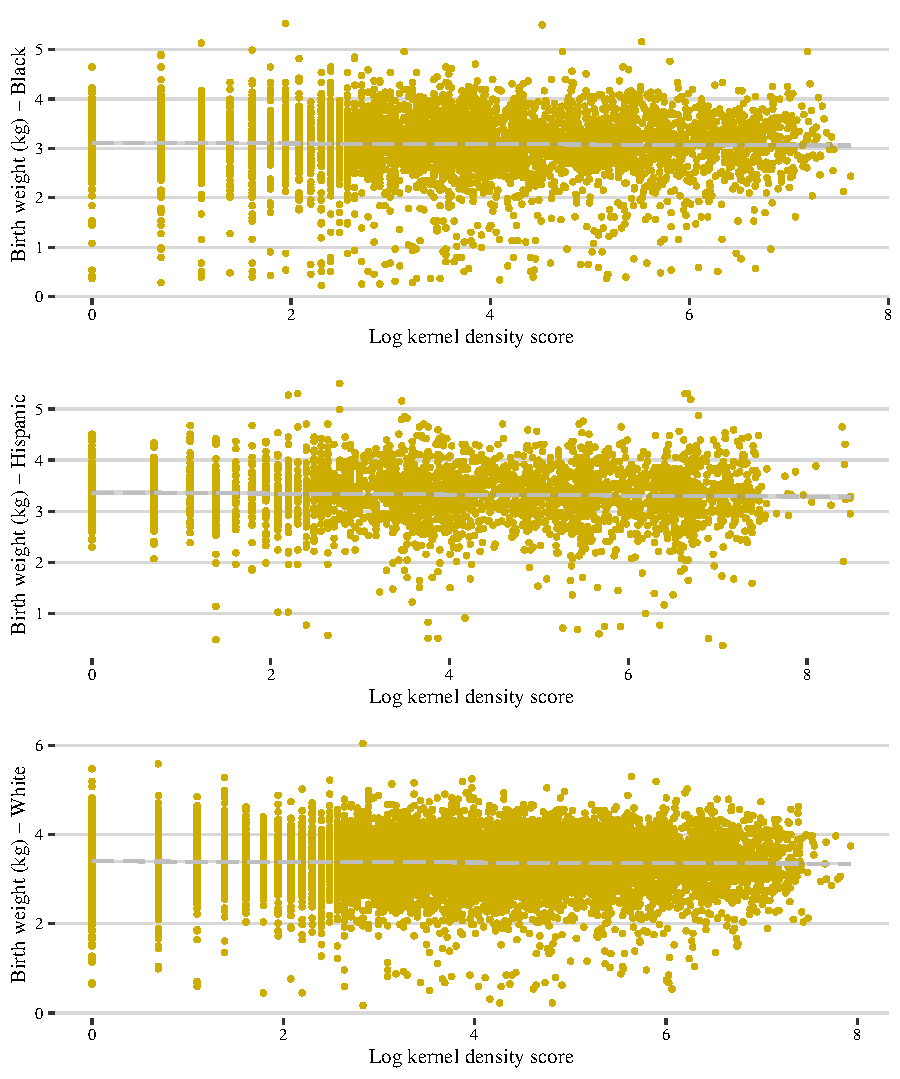
\includegraphics{ENV872_FINAL_CW_files/figure-latex/unnamed-chunk-6-1.pdf}
Figure 2: Birth weight against log kernel density score for different
race.

\begin{Shaded}
\begin{Highlighting}[]
\CommentTok{#plot}
\NormalTok{scat.gest.black <-}\StringTok{ }\KeywordTok{ggplot}\NormalTok{(df.black) }\OperatorTok{+}
\StringTok{  }\KeywordTok{geom_point}\NormalTok{(}\KeywordTok{aes}\NormalTok{(}\DataTypeTok{x =}\NormalTok{ kernel.score.log, }\DataTypeTok{y =}\NormalTok{ gestational.age), }
             \DataTypeTok{size =} \FloatTok{0.8}\NormalTok{, }\DataTypeTok{alpha =} \DecValTok{1}\NormalTok{, }\DataTypeTok{color =} \StringTok{"gold3"}\NormalTok{) }\OperatorTok{+}\StringTok{ }
\StringTok{  }\KeywordTok{geom_smooth}\NormalTok{(}\KeywordTok{aes}\NormalTok{(}\DataTypeTok{x =}\NormalTok{ kernel.score.log, }\DataTypeTok{y =}\NormalTok{ gestational.age), }
              \DataTypeTok{method =}\NormalTok{ lm, }
              \DataTypeTok{lty =} \DecValTok{5}\NormalTok{, }\DataTypeTok{lwd =} \FloatTok{0.7}\NormalTok{, }\DataTypeTok{color =} \StringTok{"gray"}\NormalTok{) }\OperatorTok{+}
\StringTok{  }\KeywordTok{labs}\NormalTok{(}\DataTypeTok{x =} \StringTok{"Log kernel density score"}\NormalTok{, }
       \DataTypeTok{y =} \StringTok{"Gestational age (weeks) - Black"}\NormalTok{) }\OperatorTok{+}
\StringTok{  }\CommentTok{#scale_color_manual(values = c("gold3", "lightskyblue3", "gray", "red3")) + }
\StringTok{  }\NormalTok{theme.hc01}

\NormalTok{scat.gest.hisp <-}\StringTok{ }\KeywordTok{ggplot}\NormalTok{(df.hisp) }\OperatorTok{+}
\StringTok{  }\KeywordTok{geom_point}\NormalTok{(}\KeywordTok{aes}\NormalTok{(}\DataTypeTok{x =}\NormalTok{ kernel.score.log, }\DataTypeTok{y =}\NormalTok{ gestational.age), }
             \DataTypeTok{size =} \FloatTok{0.8}\NormalTok{, }\DataTypeTok{alpha =} \DecValTok{1}\NormalTok{, }\DataTypeTok{color =} \StringTok{"gold3"}\NormalTok{) }\OperatorTok{+}\StringTok{ }
\StringTok{  }\KeywordTok{geom_smooth}\NormalTok{(}\KeywordTok{aes}\NormalTok{(}\DataTypeTok{x =}\NormalTok{ kernel.score.log, }\DataTypeTok{y =}\NormalTok{ gestational.age), }
              \DataTypeTok{method =}\NormalTok{ lm, }
              \DataTypeTok{lty =} \DecValTok{5}\NormalTok{, }\DataTypeTok{lwd =} \FloatTok{0.7}\NormalTok{, }\DataTypeTok{color =} \StringTok{"gray"}\NormalTok{) }\OperatorTok{+}
\StringTok{  }\KeywordTok{labs}\NormalTok{(}\DataTypeTok{x =} \StringTok{"Log kernel density score"}\NormalTok{, }
       \DataTypeTok{y =} \StringTok{"Gestational age (weeks) - Hispanic"}\NormalTok{) }\OperatorTok{+}
\StringTok{  }\CommentTok{#scale_color_manual(values = c("gold3", "lightskyblue3", "gray", "red3")) + }
\StringTok{  }\NormalTok{theme.hc01}

\NormalTok{scat.gest.white <-}\StringTok{ }\KeywordTok{ggplot}\NormalTok{(df.white) }\OperatorTok{+}
\StringTok{  }\KeywordTok{geom_point}\NormalTok{(}\KeywordTok{aes}\NormalTok{(}\DataTypeTok{x =}\NormalTok{ kernel.score.log, }\DataTypeTok{y =}\NormalTok{ gestational.age), }
             \DataTypeTok{size =} \FloatTok{0.8}\NormalTok{, }\DataTypeTok{alpha =} \DecValTok{1}\NormalTok{, }\DataTypeTok{color =} \StringTok{"gold3"}\NormalTok{) }\OperatorTok{+}\StringTok{ }
\StringTok{  }\KeywordTok{geom_smooth}\NormalTok{(}\KeywordTok{aes}\NormalTok{(}\DataTypeTok{x =}\NormalTok{ kernel.score.log, }\DataTypeTok{y =}\NormalTok{ gestational.age), }
              \DataTypeTok{method =}\NormalTok{ lm, }
              \DataTypeTok{lty =} \DecValTok{5}\NormalTok{, }\DataTypeTok{lwd =} \FloatTok{0.7}\NormalTok{, }\DataTypeTok{color =} \StringTok{"gray"}\NormalTok{) }\OperatorTok{+}
\StringTok{  }\KeywordTok{labs}\NormalTok{(}\DataTypeTok{x =} \StringTok{"Log kernel density score"}\NormalTok{, }
       \DataTypeTok{y =} \StringTok{"Gestational age (weeks) - White"}\NormalTok{) }\OperatorTok{+}
\StringTok{  }\CommentTok{#scale_color_manual(values = c("gold3", "lightskyblue3", "gray", "red3")) + }
\StringTok{  }\NormalTok{theme.hc01}

\KeywordTok{grid.arrange}\NormalTok{(scat.gest.black, scat.gest.hisp, scat.gest.white, }
             \DataTypeTok{ncol =} \DecValTok{1}\NormalTok{)}
\end{Highlighting}
\end{Shaded}

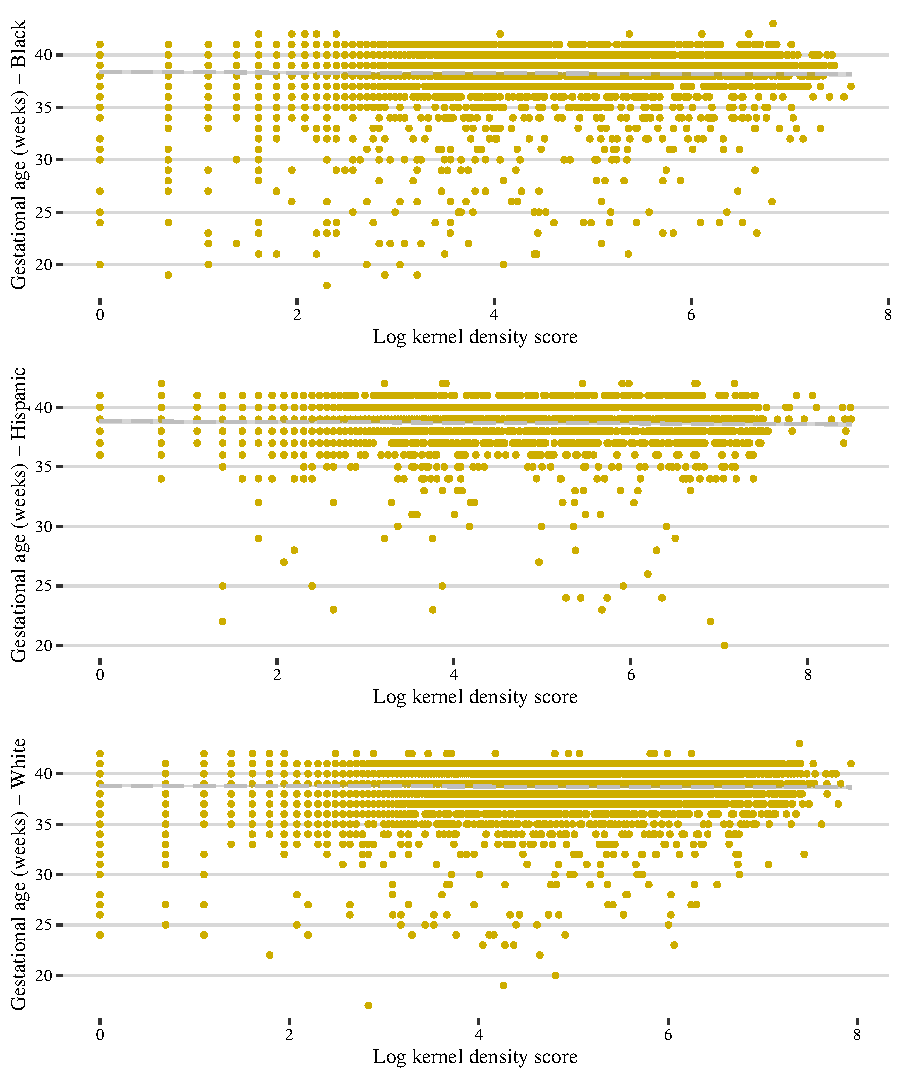
\includegraphics{ENV872_FINAL_CW_files/figure-latex/unnamed-chunk-7-1.pdf}
Figure 3: Gestational age against log kernel density score for different
race.

\newpage

\hypertarget{analysis}{%
\section{Analysis}\label{analysis}}

Generalized linear models are used to predict birth weight and
gestational age with natural log of kernel score and other confounding
variables. One log unit increase in hog CAFO kernel density score among
black and hispanic women is associated with 0.009 and 0.010 kg lower
birth weight on average (p \textless{} 0.05). One log unit increase in
kernel score among white women may be associated with 0.005 kg lower
birth weight on average, but the result is not statistically significant
(p \textgreater{} 0.05).

\begin{Shaded}
\begin{Highlighting}[]
\NormalTok{glm.birthweight.black <-}\StringTok{ }\KeywordTok{glm}\NormalTok{(}\DataTypeTok{data =}\NormalTok{ df.black, }
\NormalTok{                           birth.weight }\OperatorTok{~}\StringTok{ }\NormalTok{kernel.score.log }\OperatorTok{+}\StringTok{ }\NormalTok{infant.sex }\OperatorTok{+}\StringTok{ }\NormalTok{mother.age }\OperatorTok{+}\StringTok{ }
\StringTok{                             }\NormalTok{BMI }\OperatorTok{+}\StringTok{ }\NormalTok{education }\OperatorTok{+}\StringTok{ }\NormalTok{prenatal.care }\OperatorTok{+}\StringTok{ }\NormalTok{marital.status)}
\NormalTok{glm.birthweight.hispanic <-}\StringTok{ }\KeywordTok{glm}\NormalTok{(}\DataTypeTok{data =}\NormalTok{ df.hisp, }
\NormalTok{                           birth.weight }\OperatorTok{~}\StringTok{ }\NormalTok{kernel.score.log }\OperatorTok{+}\StringTok{ }\NormalTok{infant.sex }\OperatorTok{+}\StringTok{ }\NormalTok{mother.age }\OperatorTok{+}\StringTok{ }
\StringTok{                             }\NormalTok{BMI }\OperatorTok{+}\StringTok{ }\NormalTok{education }\OperatorTok{+}\StringTok{ }\NormalTok{prenatal.care }\OperatorTok{+}\StringTok{ }\NormalTok{marital.status)}
\NormalTok{glm.birthweight.white <-}\StringTok{ }\KeywordTok{glm}\NormalTok{(}\DataTypeTok{data =}\NormalTok{ df.white, }
\NormalTok{                           birth.weight }\OperatorTok{~}\StringTok{ }\NormalTok{kernel.score.log }\OperatorTok{+}\StringTok{ }\NormalTok{infant.sex }\OperatorTok{+}\StringTok{ }\NormalTok{mother.age }\OperatorTok{+}\StringTok{ }
\StringTok{                             }\NormalTok{BMI }\OperatorTok{+}\StringTok{ }\NormalTok{education }\OperatorTok{+}\StringTok{ }\NormalTok{prenatal.care }\OperatorTok{+}\StringTok{ }\NormalTok{marital.status)}
\KeywordTok{summary}\NormalTok{(glm.birthweight.black)}
\end{Highlighting}
\end{Shaded}

\begin{verbatim}
## 
## Call:
## glm(formula = birth.weight ~ kernel.score.log + infant.sex + 
##     mother.age + BMI + education + prenatal.care + marital.status, 
##     data = df.black)
## 
## Deviance Residuals: 
##      Min        1Q    Median        3Q       Max  
## -3.08212  -0.27669   0.05475   0.36064   2.44794  
## 
## Coefficients:
##                            Estimate Std. Error t value Pr(>|t|)    
## (Intercept)                3.117007   0.067448  46.214  < 2e-16 ***
## kernel.score.log          -0.009302   0.004559  -2.040 0.041372 *  
## infant.sexmale             0.078752   0.016257   4.844 1.31e-06 ***
## mother.age                -0.003813   0.001634  -2.333 0.019668 *  
## BMI                        0.006348   0.001029   6.167 7.44e-10 ***
## educationgraduate         -0.084817   0.055878  -1.518 0.129097    
## educationhighschool.below -0.098706   0.034037  -2.900 0.003746 ** 
## educationsome.college     -0.066419   0.033392  -1.989 0.046741 *  
## prenatal.care2             0.071317   0.034613   2.060 0.039407 *  
## prenatal.care3             0.100128   0.022925   4.368 1.28e-05 ***
## prenatal.care4            -0.070144   0.020621  -3.402 0.000675 ***
## marital.statussingle      -0.058934   0.021309  -2.766 0.005698 ** 
## ---
## Signif. codes:  0 '***' 0.001 '**' 0.01 '*' 0.05 '.' 0.1 ' ' 1
## 
## (Dispersion parameter for gaussian family taken to be 0.3716648)
## 
##     Null deviance: 2146.3  on 5632  degrees of freedom
## Residual deviance: 2089.1  on 5621  degrees of freedom
## AIC: 10424
## 
## Number of Fisher Scoring iterations: 2
\end{verbatim}

\begin{Shaded}
\begin{Highlighting}[]
\KeywordTok{summary}\NormalTok{(glm.birthweight.hispanic)}
\end{Highlighting}
\end{Shaded}

\begin{verbatim}
## 
## Call:
## glm(formula = birth.weight ~ kernel.score.log + infant.sex + 
##     mother.age + BMI + education + prenatal.care + marital.status, 
##     data = df.hisp)
## 
## Deviance Residuals: 
##      Min        1Q    Median        3Q       Max  
## -3.06256  -0.27805   0.01654   0.32228   2.03273  
## 
## Coefficients:
##                            Estimate Std. Error t value Pr(>|t|)    
## (Intercept)                2.682003   0.076625  35.002  < 2e-16 ***
## kernel.score.log          -0.010132   0.004900  -2.068   0.0387 *  
## infant.sexmale             0.134912   0.018995   7.103 1.50e-12 ***
## mother.age                 0.008962   0.001570   5.707 1.26e-08 ***
## BMI                        0.012864   0.001626   7.912 3.45e-15 ***
## educationgraduate         -0.021025   0.081360  -0.258   0.7961    
## educationhighschool.below -0.005523   0.043910  -0.126   0.8999    
## educationsome.college      0.002226   0.047058   0.047   0.9623    
## prenatal.care2             0.088074   0.037634   2.340   0.0193 *  
## prenatal.care3             0.117177   0.026128   4.485 7.56e-06 ***
## prenatal.care4            -0.060220   0.024488  -2.459   0.0140 *  
## marital.statussingle      -0.003660   0.020227  -0.181   0.8564    
## ---
## Signif. codes:  0 '***' 0.001 '**' 0.01 '*' 0.05 '.' 0.1 ' ' 1
## 
## (Dispersion parameter for gaussian family taken to be 0.2877486)
## 
##     Null deviance: 983.60  on 3198  degrees of freedom
## Residual deviance: 917.05  on 3187  degrees of freedom
## AIC: 5107.5
## 
## Number of Fisher Scoring iterations: 2
\end{verbatim}

\begin{Shaded}
\begin{Highlighting}[]
\KeywordTok{summary}\NormalTok{(glm.birthweight.white)}
\end{Highlighting}
\end{Shaded}

\begin{verbatim}
## 
## Call:
## glm(formula = birth.weight ~ kernel.score.log + infant.sex + 
##     mother.age + BMI + education + prenatal.care + marital.status, 
##     data = df.white)
## 
## Deviance Residuals: 
##    Min      1Q  Median      3Q     Max  
## -3.432  -0.295   0.013   0.344   2.568  
## 
## Coefficients:
##                            Estimate Std. Error t value Pr(>|t|)    
## (Intercept)                3.225049   0.044614  72.288  < 2e-16 ***
## kernel.score.log          -0.005209   0.003042  -1.712  0.08684 .  
## infant.sexmale             0.120412   0.010875  11.072  < 2e-16 ***
## mother.age                -0.001985   0.001151  -1.725  0.08460 .  
## BMI                        0.008493   0.000801  10.603  < 2e-16 ***
## educationgraduate          0.013000   0.021995   0.591  0.55451    
## educationhighschool.below -0.173138   0.017717  -9.773  < 2e-16 ***
## educationsome.college     -0.066819   0.015248  -4.382 1.19e-05 ***
## prenatal.care2             0.085260   0.027067   3.150  0.00164 ** 
## prenatal.care3             0.145178   0.018099   8.021 1.16e-15 ***
## prenatal.care4            -0.019000   0.016861  -1.127  0.25983    
## marital.statussingle      -0.098531   0.013340  -7.386 1.63e-13 ***
## ---
## Signif. codes:  0 '***' 0.001 '**' 0.01 '*' 0.05 '.' 0.1 ' ' 1
## 
## (Dispersion parameter for gaussian family taken to be 0.3013919)
## 
##     Null deviance: 3285.5  on 10211  degrees of freedom
## Residual deviance: 3074.2  on 10200  degrees of freedom
## AIC: 16747
## 
## Number of Fisher Scoring iterations: 2
\end{verbatim}

One log unit increase in hog CAFO kernel density score among black,
hispanic, and white women is associated with 0.042, 0.034, and 0.025
week earlier delivery on average (p \textless{} 0.05). These values
translate to 0.29, 0.27, and 0.18 days earlier. White residents living
within 5 mi from a CAFO may be less severely influenced than black and
hispanic residents.

\begin{Shaded}
\begin{Highlighting}[]
\NormalTok{glm.gestation.black <-}\StringTok{ }\KeywordTok{glm}\NormalTok{(}\DataTypeTok{data =}\NormalTok{ df.black, }
\NormalTok{                           gestational.age }\OperatorTok{~}\StringTok{ }\NormalTok{kernel.score.log }\OperatorTok{+}\StringTok{ }\NormalTok{infant.sex }\OperatorTok{+}\StringTok{ }\NormalTok{mother.age }\OperatorTok{+}\StringTok{ }
\StringTok{                             }\NormalTok{BMI }\OperatorTok{+}\StringTok{ }\NormalTok{education }\OperatorTok{+}\StringTok{ }\NormalTok{prenatal.care }\OperatorTok{+}\StringTok{ }\NormalTok{marital.status)}
\NormalTok{glm.gestation.hispanic <-}\StringTok{ }\KeywordTok{glm}\NormalTok{(}\DataTypeTok{data =}\NormalTok{ df.hisp, }
\NormalTok{                           gestational.age }\OperatorTok{~}\StringTok{ }\NormalTok{kernel.score.log }\OperatorTok{+}\StringTok{ }\NormalTok{infant.sex }\OperatorTok{+}\StringTok{ }\NormalTok{mother.age }\OperatorTok{+}\StringTok{ }
\StringTok{                             }\NormalTok{BMI }\OperatorTok{+}\StringTok{ }\NormalTok{education }\OperatorTok{+}\StringTok{ }\NormalTok{prenatal.care }\OperatorTok{+}\StringTok{ }\NormalTok{marital.status)}
\NormalTok{glm.gestation.white <-}\StringTok{ }\KeywordTok{glm}\NormalTok{(}\DataTypeTok{data =}\NormalTok{ df.white, }
\NormalTok{                           gestational.age }\OperatorTok{~}\StringTok{ }\NormalTok{kernel.score.log }\OperatorTok{+}\StringTok{ }\NormalTok{infant.sex }\OperatorTok{+}\StringTok{ }\NormalTok{mother.age }\OperatorTok{+}\StringTok{ }
\StringTok{                             }\NormalTok{BMI }\OperatorTok{+}\StringTok{ }\NormalTok{education }\OperatorTok{+}\StringTok{ }\NormalTok{prenatal.care }\OperatorTok{+}\StringTok{ }\NormalTok{marital.status)}
\KeywordTok{summary}\NormalTok{(glm.gestation.black)}
\end{Highlighting}
\end{Shaded}

\begin{verbatim}
## 
## Call:
## glm(formula = gestational.age ~ kernel.score.log + infant.sex + 
##     mother.age + BMI + education + prenatal.care + marital.status, 
##     data = df.black)
## 
## Deviance Residuals: 
##      Min        1Q    Median        3Q       Max  
## -20.4354   -0.5467    0.4528    1.2909    5.1619  
## 
## Coefficients:
##                             Estimate Std. Error t value Pr(>|t|)    
## (Intercept)               39.7110451  0.2832682 140.189  < 2e-16 ***
## kernel.score.log          -0.0419599  0.0191478  -2.191 0.028466 *  
## infant.sexmale            -0.1035856  0.0682767  -1.517 0.129287    
## mother.age                -0.0353991  0.0068627  -5.158 2.58e-07 ***
## BMI                       -0.0005979  0.0043230  -0.138 0.890002    
## educationgraduate         -0.2471556  0.2346783  -1.053 0.292309    
## educationhighschool.below -0.3096997  0.1429483  -2.167 0.030314 *  
## educationsome.college     -0.2142490  0.1402381  -1.528 0.126630    
## prenatal.care2             0.5117095  0.1453691   3.520 0.000435 ***
## prenatal.care3             0.4691546  0.0962819   4.873 1.13e-06 ***
## prenatal.care4            -0.5719678  0.0866044  -6.604 4.36e-11 ***
## marital.statussingle       0.0454597  0.0894925   0.508 0.611493    
## ---
## Signif. codes:  0 '***' 0.001 '**' 0.01 '*' 0.05 '.' 0.1 ' ' 1
## 
## (Dispersion parameter for gaussian family taken to be 6.555559)
## 
##     Null deviance: 38333  on 5632  degrees of freedom
## Residual deviance: 36849  on 5621  degrees of freedom
## AIC: 26592
## 
## Number of Fisher Scoring iterations: 2
\end{verbatim}

\begin{Shaded}
\begin{Highlighting}[]
\KeywordTok{summary}\NormalTok{(glm.gestation.hispanic)}
\end{Highlighting}
\end{Shaded}

\begin{verbatim}
## 
## Call:
## glm(formula = gestational.age ~ kernel.score.log + infant.sex + 
##     mother.age + BMI + education + prenatal.care + marital.status, 
##     data = df.hisp)
## 
## Deviance Residuals: 
##      Min        1Q    Median        3Q       Max  
## -18.5672   -0.4020    0.2875    0.8785    3.4228  
## 
## Coefficients:
##                            Estimate Std. Error t value Pr(>|t|)    
## (Intercept)               39.474977   0.266258 148.259  < 2e-16 ***
## kernel.score.log          -0.034520   0.017026  -2.027   0.0427 *  
## infant.sexmale            -0.011316   0.066003  -0.171   0.8639    
## mother.age                -0.012895   0.005457  -2.363   0.0182 *  
## BMI                       -0.003456   0.005649  -0.612   0.5407    
## educationgraduate         -0.140994   0.282711  -0.499   0.6180    
## educationhighschool.below -0.199063   0.152577  -1.305   0.1921    
## educationsome.college     -0.138897   0.163518  -0.849   0.3957    
## prenatal.care2             0.559363   0.130770   4.277 1.95e-05 ***
## prenatal.care3             0.470293   0.090790   5.180 2.36e-07 ***
## prenatal.care4            -0.442611   0.085093  -5.202 2.10e-07 ***
## marital.statussingle      -0.004815   0.070286  -0.069   0.9454    
## ---
## Signif. codes:  0 '***' 0.001 '**' 0.01 '*' 0.05 '.' 0.1 ' ' 1
## 
## (Dispersion parameter for gaussian family taken to be 3.474352)
## 
##     Null deviance: 11634  on 3198  degrees of freedom
## Residual deviance: 11073  on 3187  degrees of freedom
## AIC: 13076
## 
## Number of Fisher Scoring iterations: 2
\end{verbatim}

\begin{Shaded}
\begin{Highlighting}[]
\KeywordTok{summary}\NormalTok{(glm.gestation.white)}
\end{Highlighting}
\end{Shaded}

\begin{verbatim}
## 
## Call:
## glm(formula = gestational.age ~ kernel.score.log + infant.sex + 
##     mother.age + BMI + education + prenatal.care + marital.status, 
##     data = df.white)
## 
## Deviance Residuals: 
##      Min        1Q    Median        3Q       Max  
## -21.0557   -0.4875    0.3967    0.8584    4.4272  
## 
## Coefficients:
##                            Estimate Std. Error t value Pr(>|t|)    
## (Intercept)               39.870526   0.148101 269.211  < 2e-16 ***
## kernel.score.log          -0.025653   0.010097  -2.541 0.011080 *  
## infant.sexmale            -0.087127   0.036103  -2.413 0.015827 *  
## mother.age                -0.019674   0.003821  -5.149 2.67e-07 ***
## BMI                       -0.009226   0.002659  -3.470 0.000523 ***
## educationgraduate          0.021214   0.073014   0.291 0.771401    
## educationhighschool.below -0.373938   0.058814  -6.358 2.13e-10 ***
## educationsome.college     -0.159245   0.050617  -3.146 0.001660 ** 
## prenatal.care2             0.451236   0.089853   5.022 5.20e-07 ***
## prenatal.care3             0.530139   0.060082   8.824  < 2e-16 ***
## prenatal.care4            -0.387013   0.055973  -6.914 4.99e-12 ***
## marital.statussingle      -0.010009   0.044285  -0.226 0.821188    
## ---
## Signif. codes:  0 '***' 0.001 '**' 0.01 '*' 0.05 '.' 0.1 ' ' 1
## 
## (Dispersion parameter for gaussian family taken to be 3.321356)
## 
##     Null deviance: 35955  on 10211  degrees of freedom
## Residual deviance: 33878  on 10200  degrees of freedom
## AIC: 41253
## 
## Number of Fisher Scoring iterations: 2
\end{verbatim}

\newpage

\hypertarget{discussion-and-summary}{%
\section{Discussion and Summary}\label{discussion-and-summary}}

In general, CAFO impact level quantified by the kernel density approach
is a predictor of adverse birth outcomes (smaller gestational age \&
lower birth weight) among infants born in 2016 in NC. This project
considers other health-related confounding variables. For each log unit
change in kernel density score, black and hispanic mothers tend to be
associated with more significant change in delivery time. Black and
hispanic mothers also tend to deliver lighter infants with the same
change in kernel density scores, comparing to white mothers. This
finding adds to the belief that exposure to CAFOs is a potential
environmental justice issue. This study indicates the possibility that,
groups of minority are not only disproportionately exposed to CAFOs. At
the same time, however, they may be more vulnerable given the same level
of exposure.

\end{document}
